\section{Background}

In this section , we talk about the background knowledge of kernel TOCTOU vulnerability, how it happens. Also SMAP feature of Intel processor, how to leverage it as the core mechanism to prevent kernel TOCTOU attacks.  

TOCTOU is one category of vulnerabilities. As it's name depicts, the data has been changed since the last time it's checked. It's a problem of data inconsistency.

TOCTOU vulnerability essentially happens between protection boundary. This boundary could be implemented by hardware mechanism such as privilege levels of processors, or other protection boundary that defined and implemented by software. For example, file system provides interface that allows user to read/write file data, but if it's not integrated with  permission checking as an atomic operation, it may has TOCTOU problem.

Kernel TOCTOU is an attack that exploit TOCTOU vulnerability that found in operating system kernel components. Attackers first send in parameters which point to legit user-mode data in order to pass kernel sanity check and later replace it with a malicious one, mostly, resulting in privilege escalation. The number of such vulnerabilities has been increasing recently.

To the best of our knowledge, this is the first study that proposes a new method to mitigate kernel TOCTOU vulnerability. 

\subsection{Kernel TOCTOU/double fetch vulnerability}

Modern operating system such as Windows and Linux usually has two modes of operation, kernel mode and user mode. Operating system's kernel runs in kernel mode, it has complete access to all of the computer's hardware, and can control the switching between the CPU modes. Kernel provides most of the system's functionality including file system, network, scheduling, displaying and etc., through hundreds of "system calls". System calls provide an essential interface between a process and the operating system. The rest of the programs runs in user mode. 

User programs make system calls with parameters to get services from kernel. Those parameters could be constant number, pointers, and data structures. Top level parameters will be copied from user stack to kernel stack by the system call dispatcher, because of that, they are not changeable. But there are parameters that contains sub-level pointers which points to user-mode memory. Operating system may references those when handling a system call. It's not guaranteed by any system mechanism and those data can be modified by other threads at anytime.

Therefore, it's dangerous for the kernel to reference any user-mode data directly, especially, more than once. Kernel should first make it's own copy of which it's about to use and keep using the copy instead of the original one though the entire system call, otherwise attackers can just send in parameters that look legit to pass kernel's sanity check and later replace it with malicious ones.

The number of kernel TOCTOU vulnerability has been increasing recently. For example, the kernel mode graphic subsystem of Windows operating system, It interacts with user-mode variables frequently. The following table is the vulnerabilities that found in recent years.

\begin{comment}


\begin{table}[]
\centering
\caption{My caption}
\label{my-label}
\begin{tabular}{|l|l|l|l|}
\hline
CVE-2013-1248 & CVE-2013-1258 & CVE-2013-1268 & CVE-2013-1279 \\
CVE-2013-1249 & CVE-2013-1259 & CVE-2013-1269 & CVE-2013-1280 \\
CVE-2013-1250 & CVE-2013-1260 & CVE-2013-1270 & CVE-2015-6101 \\
CVE-2013-1251 & CVE-2013-1261 & CVE-2013-1271 & CVE-2010-1888 \\
CVE-2013-1252 & CVE-2013-1262 & CVE-2013-1272 & CVE-2008-2252 \\
CVE-2013-1253 & CVE-2013-1263 & CVE-2013-1273 & CVE-2017-11830 \\
CVE-2013-1254 & CVE-2013-1264 & CVE-2013-1275 &  \\
CVE-2013-1255 & CVE-2013-1265 & CVE-2013-1276 &  \\
CVE-2013-1256 & CVE-2013-1266 & CVE-2013-1277 &  \\
CVE-2013-1257 & CVE-2013-1267 & CVE-2013-1278 &  \\ \hline
\end{tabular}
\end{table}
\end{comment}


\begin{comment}

% Please add the following required packages to your document preamble:
% \usepackage{graphicx}
\begin{table}[tp]
\centering
\resizebox{\columnwidth}{!}{%
\begin{tabular}{|l|l|}
\hline
CVEs & Description \\ \hline
CVE-2008-2252 & \begin{tabular}[c]{@{}l@{}}Microsoft Security Bulletins MS08-061 \\ addressed 32 Elevation of Privilege issues.\\ Race condition vulnerabilities found in win32k.sys\\ Affected systems: Windows XP, Windows 2008\end{tabular} \\ \hline
CVE-2010-1888 & \begin{tabular}[c]{@{}l@{}}Addressed in Microsoft Security Bulletins MS10-047,\\ a race condition vulnerability found in win32k.sys.\\ Affected systems: from Windows XP to Windows 2008\end{tabular} \\ \hline
\begin{tabular}[c]{@{}l@{}}CVE-2013-1248\\ ...\\ CVE-2013-1280\end{tabular} & \begin{tabular}[c]{@{}l@{}}Microsoft Security Bulletins MS13-016 and MS13-\\ 017 addressed 32 Elevation of Privilege issues.\\ Race condition vulnerabilities found in win32k.sys\\ Affected systems: from Windows XP to Windows 2008\end{tabular} \\ \hline
\begin{tabular}[c]{@{}l@{}}CVE-2013-1283\\ CVE-2013-1284\\ CVE-2013-1291\\ ...\\ CVE-2013-1294\end{tabular} & \begin{tabular}[c]{@{}l@{}}Microsoft Security Bulletins MS13-031 and MS13-036\\ addressed six Elevation of Privilege issues.\\ Race condition vulnerabilities found in win32k.sys\\ Affected systems: from Windows XP to Windows 2012\end{tabular} \\ \hline
CVE-2015-6101 & \begin{tabular}[c]{@{}l@{}}Addressed in Microsoft Security Bulletins MS15-115, \\ a race condition vulnerability found in win32k.sys\\ Affected systems: from Windows XP to Windows 2012\end{tabular} \\ \hline
\end{tabular}%
}
\caption{Description of Identified Kernel TOCTOU (Double Fetch) Vulnerabilities}
\label{table:vulnerabilities}
\end{table}

\end{comment}

% Please add the following required packages to your document preamble:
% \usepackage{graphicx}
\begin{table*}[ht]
\centering
\resizebox{\textwidth}{!}{%
\begin{tabular}{lll}
\hline
CVEs & Affected Systems(*) & Description \\ \hline
CVE-2008-2252 & \begin{tabular}[c]{@{}l@{}}Windows 2000 sp4\\ Windows XP sp2, sp3\\ Windows 2003 sp2, sp3\\ Windows Vista rtm, sp1\\ Windows 2008\end{tabular} & A kernel TOCTOU(double fetch) vulnerability in the function xxxInterSendMessageEx of module win32k.sys. Addressed in Microsoft Security Bulletins MS08-061. \\ \hline
\begin{tabular}[c]{@{}l@{}}CVE-2013-1248\\ ...\\ CVE-2013-1280\end{tabular} & \begin{tabular}[c]{@{}l@{}}Windows XP sp3\\ Windows 2003 sp2\\ Windows Vista sp2\\ Windows 7 rtm, sp1\\ Windows 2008 sp2\end{tabular} & \begin{tabular}[c]{@{}l@{}}Thirty kernel TOCTOU(double fetch),vulnerabilities which have the same flaw code among functions CalcOutputStringSize, ClientGetListboxString, ClientGetMessageMPH,\\  ClientImmLoadLayout,CopyOutputString,SfnINOUTDRAG, SfnINOUTLPMEASUREITEMSTRUCT, SfnINOUTLPPOINT5,SfnINOUTLPRECT, SfnINOUTLPSCROLLINFO,\\  SfnINOUTLPUAHMEASUREMENUITEM, SfnINOUTLPWINDOWPOS, SfnINOUTNEXTMENU, SfnINOUTSTYLECHANGE, SfnOUTLPCOMBOBOXINFO, SfnOUTLPRECT,\\  SfnOUTLPSCROLLBARINFO,SfnOUTLPTITLEBARINFOEX, fnHkINDWORD, fnHkINLPCBTCREATESTRUCT,fnHkINLPMOUSEHOOKSTRUCTEX, fnHkINLPRECT,\\  fnHkOPTINLPEVENTMSG, xxxClientCopyDDEIn1, xxxClientCopyDDEOut1,xxxClientGetCharsetInfo,xxxClientGetDDEHookData in moudlewin32k.sys.\\  Addressed in Microsoft Security Bulletins MS13-016 and MS13-017.\end{tabular} \\ \hline
\begin{tabular}[c]{@{}l@{}}CVE-2013-1283\\ CVE-2013-1284\\ CVE-2013-1291\\ ...\\ CVE-2013-1294\end{tabular} & \begin{tabular}[c]{@{}l@{}}Windows XP sp3\\ Windows 2003 sp2\\ Windows Vista sp2\\ Windows 7 rtm, sp1\\ Windows 2008 sp2\end{tabular} & Race condition vulnerabilities found in win32k.sys. Addressed in Microsoft Security Bulletins MS13-031 and MS13-036. \\ \hline
\end{tabular}%
}
\caption{Description of Identified Kernel TOCTOU (Double Fetch) Vulnerabilities. (*)Partially listed}
\label{my-label}
\end{table*}

%\caption{Description of Identified Kernel TOCTOU (Double Fetch) Vulnerabilities. (*)Partially listed}


Notice that large part of the vulnerabilities of this table (from CVE-2013-1248 to CVE-2013-1280) are fixed in one Windows patch MS13-016, they are found by Gynvael Coldwind and Mateusz Jurczyk with Google Security Team. Due to the nature of kernel TOCTOU, it's difficult to exposure them in normal ways of testing or daily usage, until certain pattern and methods are found~\cite{jurczyk2013identifying}.  

\begin{comment}
\begin{figure}[th]
  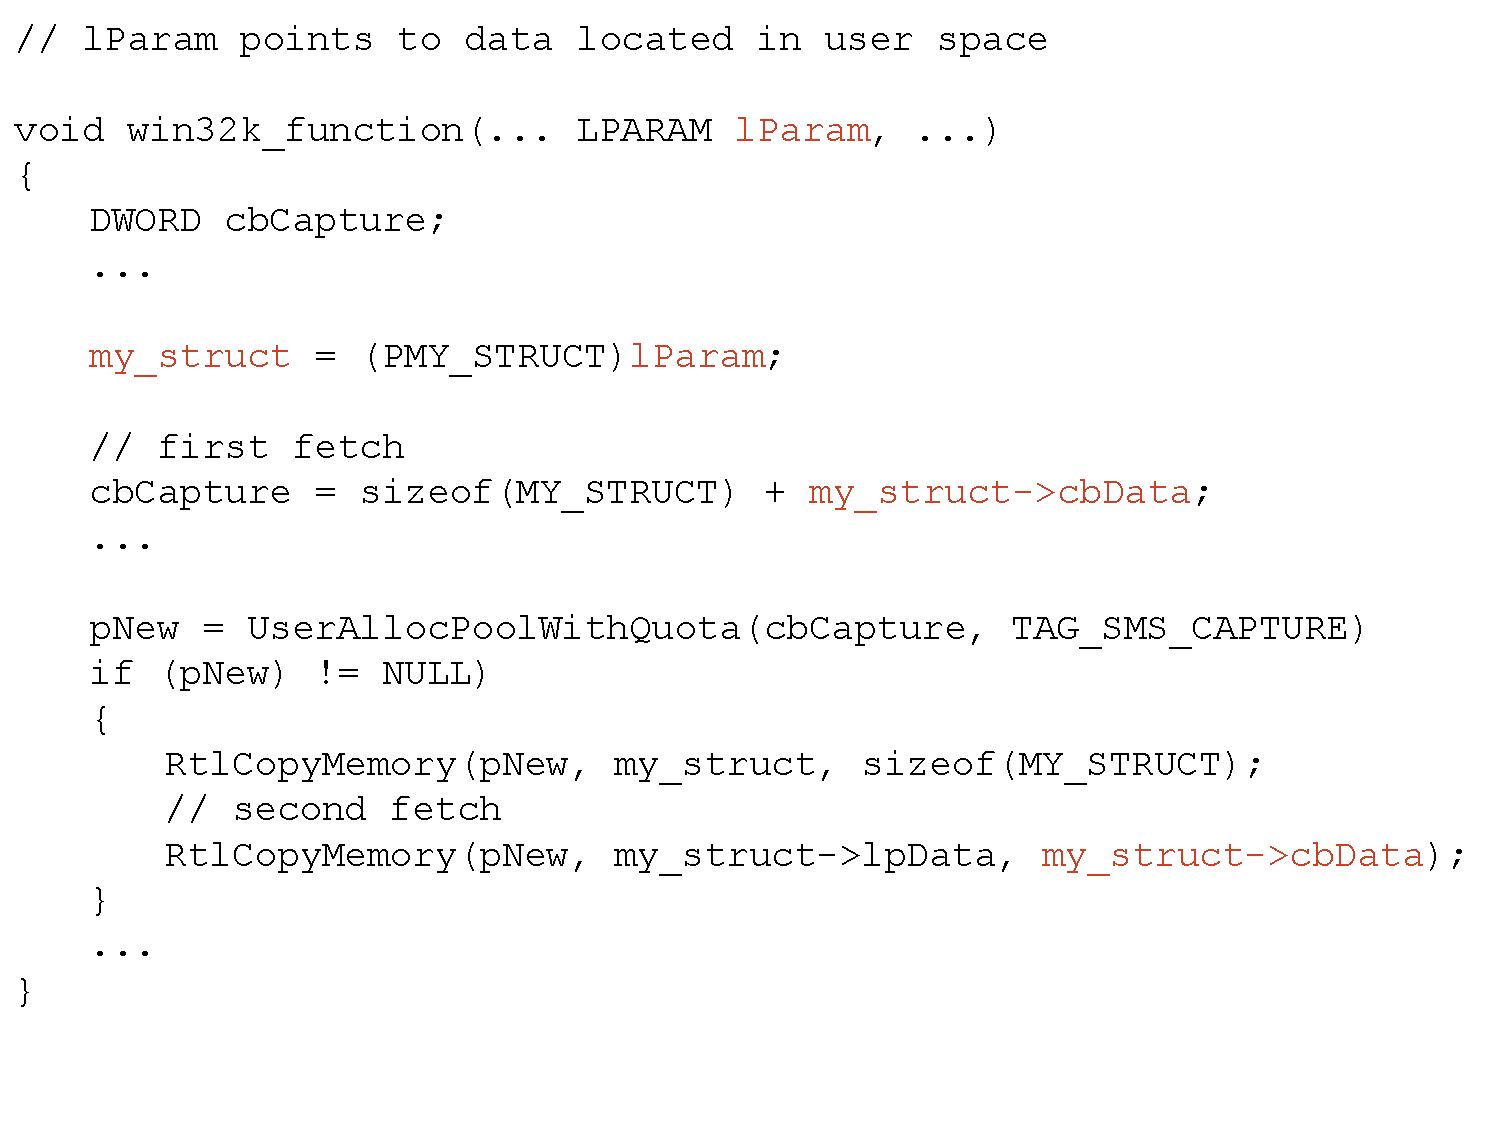
\includegraphics[width=0.47\textwidth]{toctouexample}
  \centering
  \caption{Sample code which has TOCTOU vulnerability. Data with in user space is referenced twice during a kernel pool allocation and data copying. ~\cite{jurczyk2013identifying}~\cite{ms08061}}
  \label{fig:toctouexample}
\end{figure}
\end{comment}


%lst:vulnerablecode
\begin{lstlisting}[basicstyle=\small,style=base,caption={An snippet of Windows device driver code that mimic the vulnerability that fixed in ms08-061. The vulnerable user-mode variable is marked in red.}\label{lst:vulnerablecode}]

// lParam points to data located in user space

void win32k_function(... LPARAM @lParam@, ...) 
{
    DWORD cbCapture;
    ...

    @my_struct@ = (PMY_STRUCT)@lParam@;

    // first fetch
    cbCapture = sizeof(MY_STRUCT) + @my_struct->cbData@;  
    ...

    pNew = UserAllocPoolWithQuota(cbCapture, TAG_SMS_CAPTURE)
    if (pNew != NULL) 
    {
        RtlCopyMemory(pNew, my_struct, sizeof(MY_STRUCT);
        // second fetch
        RtlCopyMemory(pNew, my_struct->lpData, @my_struct->cbData@);   
    }
    ...
}

\end{lstlisting}

Listing~\ref{lst:vulnerablecode} shows an snippet of Windows device driver code~\cite{jurczyk2013identifying} that a buffer first allocated from kernel heap, whose size is determined from a variable resides in user-mode, and later reuses that variable as a parameter in a "RtlCopyMemory" call. This is a piece of pseudo code that mimic the vulnerability that has been patched in ms08-061. "my_struct-$>$cbData" appears two times, referencing user-mode variable, one is to determine the size of the kernel buffer (first fetch), the other is to use it as the length of data(second fetch). Since variable resides in user-mode memory could be modified by other threads, later, "my_struct-$>$cbData" could be set to a larger value, introducing a potential kernel pool buffer overflow.

This attack can happen on both single processor system and multiple processor system. On a single processor system, even though only one thread can be scheduled to execute on the processor at a time, it's still possible to trigger the vulnerability. For example, between function calls UserAllocPoolWithQuota and RtlCopyMemory, if a thread context switch happens in between, other threads can have the opportunity to modified it.

A multiple processor environment is much more favorable to attackers. It's commonplace for both laptops or servers nowadays. Under such conditions, the attacker creates an attacking thread and use thread affinity masks to attach it to other processors. As shown in~\autoref{fig:toctouasm}. The attacking thread keeps flipping the vulnerable variable in a loop, high chance that it can successfully enlarge it during the time window. In this paper we assume the attacker captures the time window and corrupts the vulnerable value as intended. 

\begin{figure}[h]
  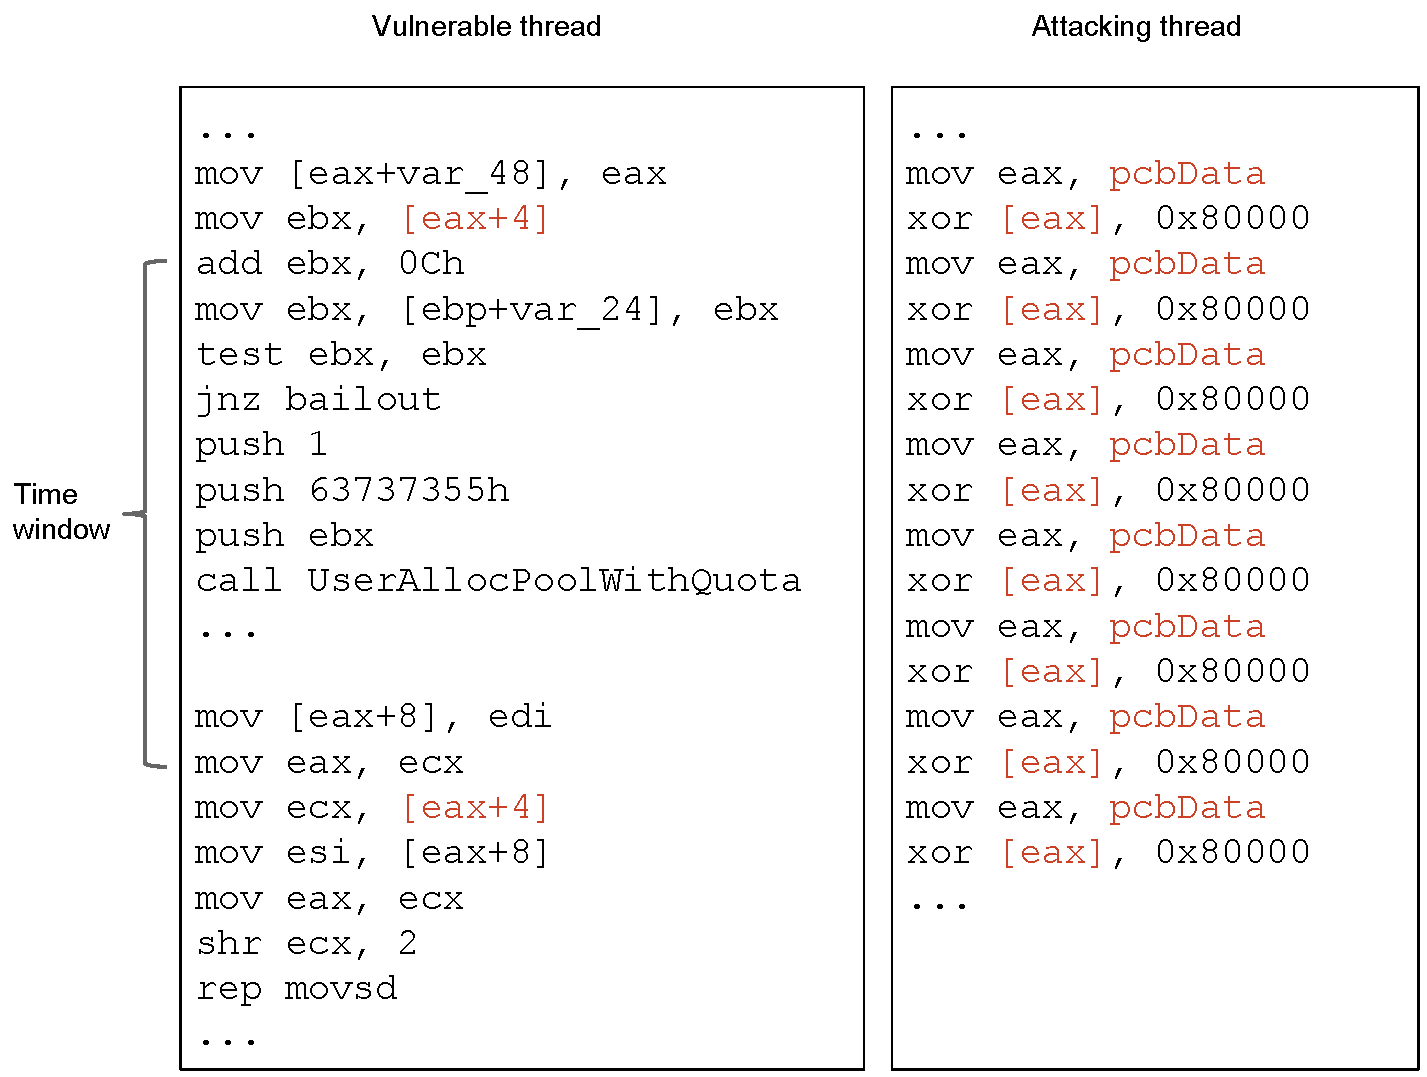
\includegraphics[width=0.47\textwidth]{toctouasm}
  \centering
  \caption{The attacking thread could be as simple as several instructions in a loop.}
  \label{fig:toctouasm}
\end{figure}


\subsection{Supervisor Mode Access Prevention (SMAP)}
SMAP is a security feature of Intel processors since Broadwell microarchitecture. It prevents operating system kernel accessing user-mode memory directly, such accesses will raise an exception. This makes it harder for attackers to "trick" the kernel into using instructions or data from a user-mode program. 

Kernel code reads and writes user-mode data are commonplace. It's inevitable because user programs need to provide parameters to system calls. Therefore, two new instructions "STAC" and "CLAC" are provided to disable SMAP temporarily, giving opportunity for kernel to retrieve user data in a controllable way.

Linux kernel support for SMAP since version 3.7. All the accesses to user mode memory must go through two gateway functions copy_to_user() and copy_from_user(), where SMAP is temporarily disabled.

Windows doesn't support SMAP yet. Different from Linux's approach, each of Windows system calls tends to "probe" and "capture" user-mode data itself. Probing usually done by function ProbeForRead()~\cite{probeforread} and ProbeForWrite() to check the validity of the buffers, it also checks if a user-mode buffer actually resides in the user-mode address space by simply compare its address to a pre-defined value. Since some modules such as win32k.sys are highly coupled with user-mode components, it will cost huge engineering effort to change the way it retrieve user-mode data.

In Linux, even though copy_*_user() is mandated~\cite{corbet2012linuxsmap}, it still suffers from TOCTOU vulnerability such as mistake of using function copy_from_user() twice for the same variable~\cite{double-fetch-linux}. 